\chapter{Introduction}

\epigraph{``And now you're asking, I don't know where to begin''}{{\sl Mike Vennart, Silent/Transparent}}
%
%“We demand rigidly defined areas of doubt and uncertainty!” 
%― Douglas Adams, The Hitchhiker's Guide to the Galaxy

The release of gravitational potential energy as mass falls towards
a compact object is the most efficient energetic process in the universe,
capable of liberating more rest mass energy than nuclear fusion.
This {\em accretion} process is thought to power the huge radiative engines at the 
centres of every galaxy -- accreting supermassive black holes known as active galactic nuclei (AGN). 
In addition to AGN, accretion discs are seen in X-ray binaries (XRBs), young-stellar objects (YSOs) and
accreting white dwarfs (AWDs). Accretion therefore appears to be a universal process; broadly speaking, the physics is similar whether it is taking place in a $\sim1~M_\odot$ Neutron Star or White Dwarf 
system, or a $\sim10^{10}~M_\odot$ black hole -- a {\em quasar}. 

Outflows are ubiquitous in accreting systems. We see collimated radio jets in AGN (REF) and
XRBs (REF), and there is even evidence of extended radio emission in AWDs (REF). These radio jets
tend to appear in specific accretion states (REF), implying an intrinsic connection to the 
accretion process. Even more intriguing, in XRBs less collimated, mass-loaded outflows
or {\em winds} are observed in the opposite accretion state, possibly emanating from the accretion disc.
Evidence for disc winds is widespread across the mass range, but perhaps the most spectacular indication
is the blue-shifted, broad absorption lines (BALs) in the rest-frame ultraviolet (UV)
seen in high-state AWDs (REFs) and so-called broad absorption line quasars seen in $20-40\%$
of quasars (BALQSOs; REFs). 

The astrophysical significance of disc winds extends, quite literally, 
far beyond the accretion environment. They offer a potential mechanism by which the central
accretion engine can interact with the host galaxy and interstellar medium (REFs). 
This is often referred to as AGN feedback (REF), and is required in models of 
galaxy evolution

This thesis is structured as follows. In the remainder of this chapter, 
I shall describe the different classes of accreting systems and give a history
of their study. In chapter 2, I will give the background accretion theory 
and detail the successes and failures of accretion disc models when compared to observations, before 
discussing the outflows associated with accretion discs in chapter 3. Chapter 4
outlines the Monte Carlo radiative transfer (MCRT) and photoionization
methods I have used in order to investigate the impact of disc 
winds on the spectra of accreting systems. The science chapters
contain three separate submitted papers, in which we investigated the impact
of disc winds on the spectra of CVs (Chapter 5), and tested the disc winds
quasar unification model (Chapters 6 and 7).
In chapter 8, I summarise my findings and their astrophysical significance, 
and discuss potential avenues for future work.

\section{Accreting Compact Binaries}

\subsection{Cataclysmic Variables}
Cataclysmic variables (CVs) are systems in which a white dwarf
accretes matter from a donor star via Roche-lobe overflow. In
non-magnetic systems this accretion is mediated by a Keplerian disc
around the white dwarf (WD). Nova-like variables (NLs) are a subclass
of CVs in which the  disc is always in a relatively
high-accretion-rate state ($\dot{M} \sim 10^{-8}$~M$_{\odot}$~yr$^{-1}$).  
This makes NLs an excellent laboratory for studying the properties of 
steady-state accretion discs. 

\subsection{X-ray Binaries}
X-ray binaries are similar to CVs in structure, except that the compact object
is either a neutron star (NS) or black hole (BH). The accretion disc 
emits in the soft X-rays, and an additional hard X-ray power law is also 
seen in the spectrum (REFs). This hard component is normally attributed
to Compton up-scattering of seed disc photons by some kind of `corona'
of hot electrons close to the BH (REFs). 

Although I do not discuss XRBs directly in this thesis, it is instructive
to discuss some of their observational appearance as it is instructive 
for understanding the theory of disc winds, as well as their wider significance. 
The discovery that XRBs follow similar tracks on a hardness-intensity diagram (REFs)
is particularly interesting in this regard, especially since Ponti et al. (2012)
showed that broad Fe absorption lines are only seen in the soft-state 
high-inclination systems, implying that equatorial outflows are intrinsic to 
the accretion process (see figure~\ref{fig:ponti_cartoon}). Although the driving mechanism
is almost certainly different to CVs (REFs), the similarity in general structure 
to models for CVs and quasars is striking.

\begin{figure}
\centering
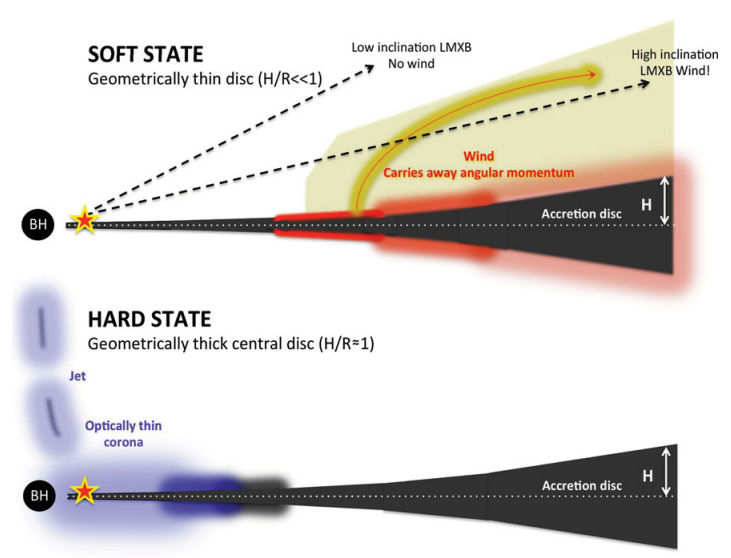
\includegraphics[width=0.7\textwidth]{figures/01-intro/ponti_wind_cartoon.png}
\caption
[Hardness intensity diagram for a WD, NS and BH system]
{
{\sl Credit: Ponti et al. 2012}
Hardness intensity diagram for a WD, NS and BH system
} 
\label{fig:ponti_cartoon}
\end{figure}




\section{Quasars and Active Galactic Nuclei}

Spectra of AGN have now been studied for over 100 years, and we have known 
that they exhibit strong, broad emission lines since the first spectrum was taken by
\cite{fath1909}.
However, it wasn't until the work of \cite{seyfert1943} that the systematic 
classification of AGN really began, leading to the phrase `Seyfert galaxy'.
This label was applied to galaxies possessing a bright nucleus, spectroscopically
characterised by a blue continuum and a series of strong emission lines.
The first real physical insight into the extraordinary nature of AGN
was provided by \cite{woltjer1959}, who noted that (i) the nuclei must have sizes $<100$~pc,
based on the fact that they were unresolved and (ii) the mass of the nucleus
must be very high, based on virialised motion. 
While both of these observations were based on simple arguments, the fact that these
ultra-luminous celestial objects are both {\em compact} and {\em supermassive}
is perhaps the defining insight into the nature of AGN.

Although the field of AGN study was established in the optical, 
radio astronomy also significantly furthered our understanding of AGN
in the mid-20th century. A number of surveys, such as the Cambridge \citep{edge1959}, 
Parkes \citep{ekers1969} and Ohio \citep{ehman1970} surveys discovered a great many 
bright radio point sources distributed isotropically across the sky.
These sources eventually became known as `quasi-stellar radio sources'
or {\em quasars}, and were soon identified to be coincident with bright optical
sources or `quasi-stellar objects' (QSOs; REFs). 
Nowadays, the term quasar normally has very little to do with 
radio emission and is often used interchangeably with QSO. 
Indeed, throughout this thesis I shall refer to a quasar as simply a bright, 
massive AGN; one with sufficiently high luminosity that it dominates the emission 
from it's host galaxy. 



\subsection{AGN Unification and the dusty Torus}

NGC 1068 

\subsection{The Broad Line Region}




\subsection{Broad Absorption: Evidence of winds}


\subsection{Disc Wind Unification Pictures}

As noted by \cite[][hereafter MCGC95]{MCGV95}, there are a number of problems with
the BLR `cloud' model, perhaps most notably that there is no obvious 
physical origin for a series of virialised clouds. While there are exceptions
to this statement (REFs), it is important to test other models.
Indeed, MCGV95 proposed a disc wind model in order to explain both BALs and BELs
in quasars. A disc wind model was also  discussed by \cite{elvis2000}, 
who proposed a structure for quasars that attempted to explain much 
of the behaviour of luminous AGN
merely as a function of viewing angle. Outflow models are discussed further in section~?.
The philosophy of these models is that, before invoking additional
degrees of freedom in a model, we should first test if known quasar phenomenology 
(winds) can explain other aspects of their observational appearance.
I have illustrated this general principle with the `Occam's quasar' 
cartoon shown in figure~\ref{fig:occam}. This is the picture that I will
to test in the latter, quasar-focused sections of this thesis, and the general
principle can even be applied to cataclysmic variables and other accreting objects.



\begin{figure}
\centering
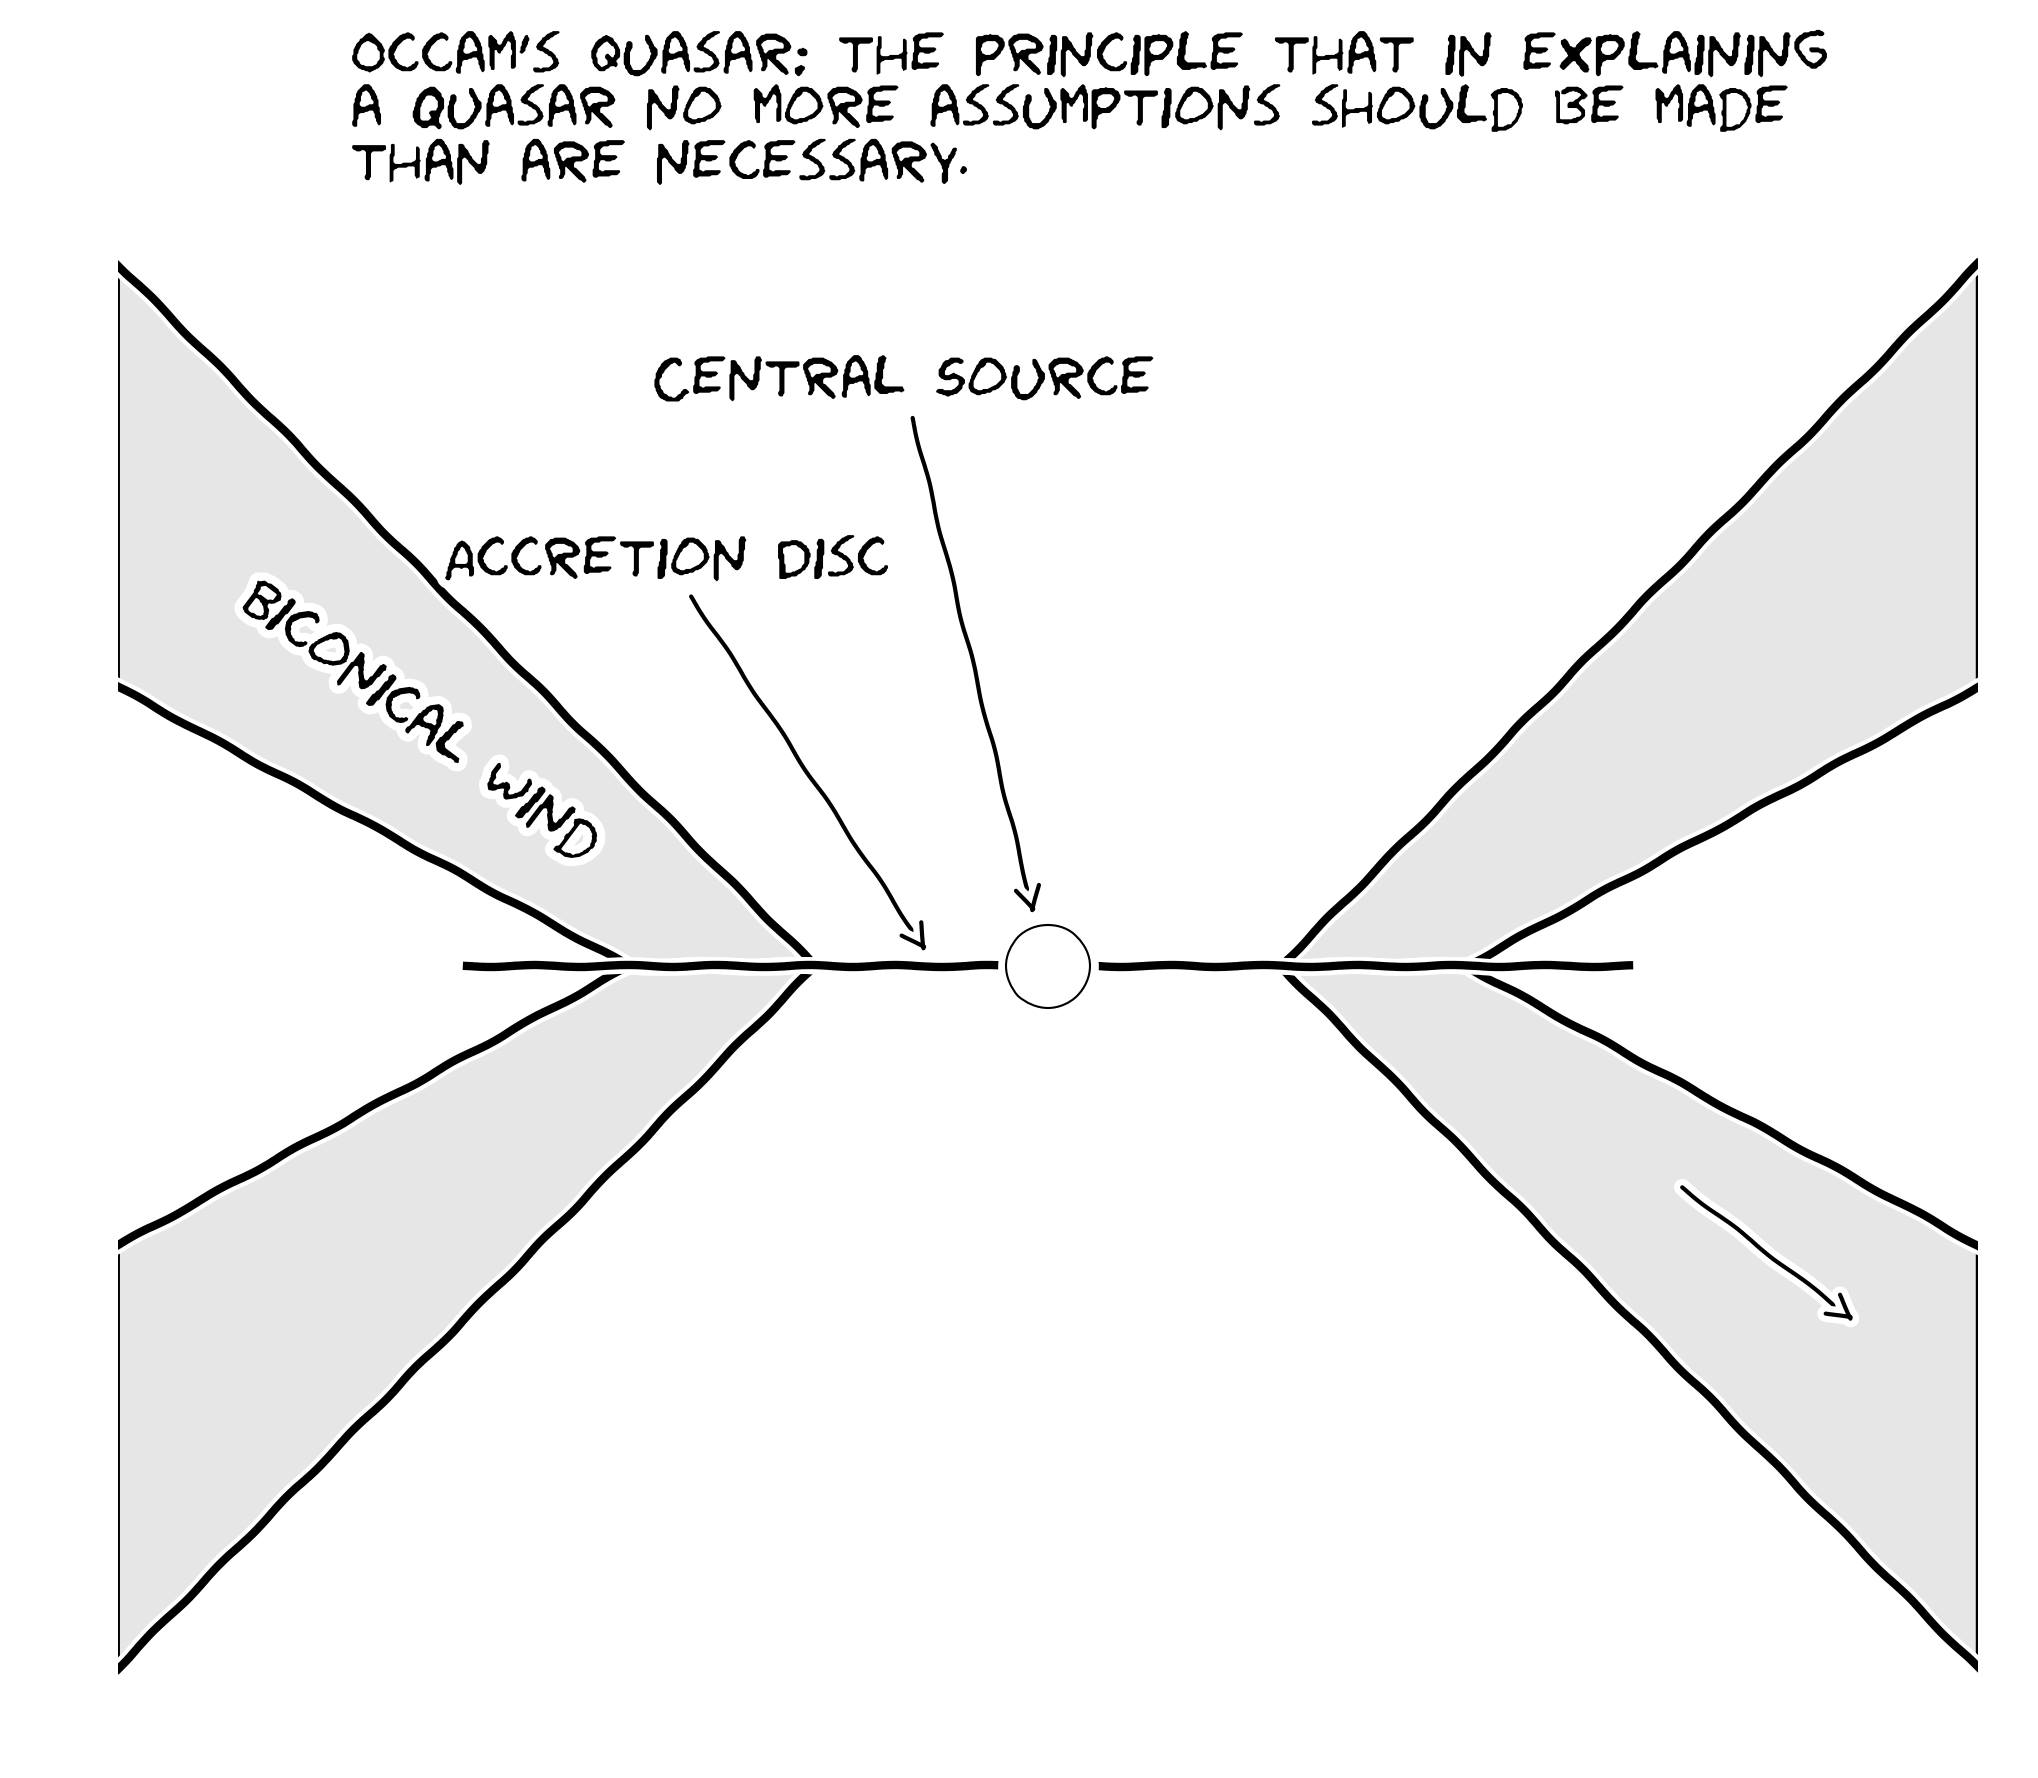
\includegraphics[width=1.0\textwidth]{figures/01-intro/occam.jpg}
\caption
[Occam's quasar]
{
Occam's quasar. How far can this general picture take us when trying to explain
the behaviour of quasars and other accreting compact objects?
} 
\label{fig:occam}
\end{figure}

